\documentclass[11pt,a4paper]{article}
\usepackage{fontspec}
\usepackage{amsmath,amssymb}
\usepackage{tikz}
\usepackage{geometry}
\geometry{margin=18mm,top=20mm,bottom=20mm}
\usepackage{fancyhdr}
\usepackage[hidelinks]{hyperref}
\usepackage{xurl}
\definecolor{ink}{HTML}{182D3D}
\color{ink}
\pagestyle{fancy}\fancyhf{}\fancyhead[L]{\small ISEGORIA / INTEGRATION}\fancyhead[R]{\small 14 September 2026}\fancyfoot[R]{\thepage\ / 5}
\setlength{\parindent}{0pt}\setlength{\parskip}{7pt}
\newcommand{\topic}[1]{\vspace{6pt}{\large\bfseries #1}\par}
\newcommand{\pagetitle}[1]{{\LARGE\bfseries #1}\par\vspace{9pt}}
\setmainfont{Palatino}
\begin{document}
\pagetitle{Lebesgue vs Riemann integration}

Riemann groups nearby inputs. Lebesgue groups equal or similar outputs, then measures where they occur. Explore how both recover the same area, and where their definitions part company.

\begin{center}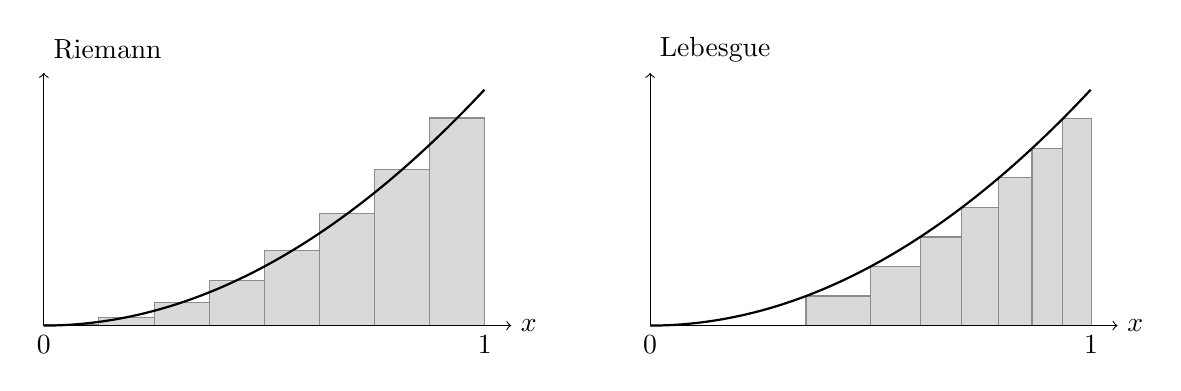
\begin{tikzpicture}[x=5.6cm,y=3.0cm]
\begin{scope}
\node[anchor=west] at (0,1.17) {Riemann};
\foreach \i in {0,...,7}{\pgfmathsetmacro{\a}{\i/8}\pgfmathsetmacro{\b}{(\i+1)/8}\pgfmathsetmacro{\h}{((\i+.5)/8)^2}\filldraw[fill=black!15,draw=black!45] (\a,0) rectangle (\b,\h);}
\draw[->] (0,0)--(1.06,0) node[right] {$x$};\draw[->](0,0)--(0,1.07);\draw[thick,domain=0:1,samples=70] plot (\x,{\x*\x});\node[below]at(0,0){$0$};\node[below]at(1,0){$1$};
\end{scope}
\begin{scope}[xshift=7.7cm]
\node[anchor=west] at (0,1.17) {Lebesgue};
\foreach \i in {0,...,7}{\pgfmathsetmacro{\a}{sqrt(\i/8)}\pgfmathsetmacro{\b}{sqrt((\i+1)/8)}\pgfmathsetmacro{\h}{\i/8}\filldraw[fill=black!15,draw=black!45] (\a,0) rectangle (\b,\h);}
\draw[->](0,0)--(1.06,0) node[right]{$x$};\draw[->](0,0)--(0,1.07);\draw[thick,domain=0:1,samples=70] plot (\x,{\x*\x});\node[below]at(0,0){$0$};\node[below]at(1,0){$1$};
\end{scope}\end{tikzpicture}\end{center}

\topic{What the pictures are actually saying}

Riemann fixes a partition \(a=x_0<\cdots<x_n=b\), chooses \(\xi_i\) in each subinterval, and forms S. A bounded function is Riemann integrable when all tagged sums approach the same finite value as the largest interval width tends to zero. One successful sequence of midpoint sums is not enough.

\[S(P,f)=\sum_{i=1}^n f(\xi_i)(x_i-x_{i-1}).\]

Lebesgue starts with a nonnegative measurable simple function \(s=\sum_k a_k\mathbf{1}_{E_k}\) on disjoint measurable sets \(E_k\). Its integral is \(\sum_k a_k\mu(E_k)\). The sets need not be intervals. For measurable \(f\ge0\), define \(\int f\,d\mu\) as the supremum of \(\int s\,d\mu\) over all simple functions with \(0\le s\le f\). The value may be infinite.

\[\int f\,d\mu=\sup_{0\le s\le f,\ s\text{ simple}}\int s\,d\mu.\]

\newpage

\pagetitle{Exact examples and error bounds}

In this lab, \(0\le f\le1\) and each value band has width \(\frac1n\). The final band includes the value 1. Thus \(0\le f-s\le 1/n\) on a domain of measure 1, so \(\int s\,d\mu\le\int f\,d\mu\le\int s\,d\mu+\frac1n\). Refinement uses nested dyadic bands. Set lengths are analytic; displayed numbers are rounded.

\topic{$f(x)=x^2$, $n=4$}

The midpoint sum is\[\frac{(1/8)^2+(3/8)^2+(5/8)^2+(7/8)^2}{4}=\frac{21}{64}=0.328125,\qquad \int_0^1x^2\,dx=\frac13.\]

The preimage of a value band and its measure are

\[E_k=\left[\sqrt{\frac{k}{n}},\sqrt{\frac{k+1}{n}}\right),\quad \mu(E_k)=\sqrt{\frac{k+1}{n}}-\sqrt{\frac{k}{n}}.\]

Include the right endpoint in the final interval. \[\int s_4\,d\mu=\sum_{k=0}^3\frac{k}{4}\left(\sqrt{\frac{k+1}{4}}-\sqrt{\frac{k}{4}}\right)\approx0.231717.\]

\topic{$f(x)=1-|2x-1|$}

Up to endpoints, the preimage of a value band consists of two intervals:

\[\left[\frac a2,\frac b2\right]\cup\left[1-\frac b2,1-\frac a2\right],\qquad \mu(E)=b-a.\]

Consequently,\[\int s_n\,d\mu=\frac{n-1}{2n},\qquad \int_0^1f(x)\,dx=\frac12.\]

\topic{A related picture: horizontal layers}

For nonnegative measurable f, the layer-cake identity is \(\int f\,d\mu=\int_0^\infty\mu(\{x:f(x)>t\})\,dt\). This adds thickness × length of a superlevel set. It is equivalent to the integral, but is distinct from weighting disjoint value bands by their lower values. Lebesgue integration is not merely exchanging x and y.

\newpage

\pagetitle{Where Riemann stops}

Let \(D(x)=1\) when x is rational, and \(D(x)=0\) when x is irrational, on \([0,1]\). This is a definition, not a curve a computer can faithfully plot.

\[D(x)=\mathbf1_{\mathbb Q\cap[0,1]}(x)=\begin{cases}1&x\in\mathbb Q,\\0&x\notin\mathbb Q.\end{cases}\]

Every lower Darboux sum is 0; every upper Darboux sum is 1. Rational tags produce a sum of 1 and irrational tags a sum of 0 at every resolution. There is no Riemann integral.

\[L(P,D)=0\ne1=U(P,D),\qquad \int D\,d\mu=0.\]

The rationals in \([0,1]\) are countable, and each singleton has Lebesgue measure zero. Countable additivity gives \(\mu(\mathbb Q\cap[0,1])=0\). Therefore \(\int D\,d\mu=1\cdot0=0\).

\topic{Measure zero does not mean empty}

Enumerate the rationals as \(q_1,q_2,\ldots\) . Given \(\varepsilon>0\), cover \(q_j\) by an interval of length \(\varepsilon/2^j\). The union covers every rational and its total length is at most \(\varepsilon\). Since \(\varepsilon\) is arbitrary, the set has measure zero. Density and measure answer different questions.

\topic{When they agree}

A bounded function on a compact interval is Riemann integrable if and only if its discontinuities form a set of Lebesgue measure zero. Whenever it is Riemann integrable, it is Lebesgue integrable with the same value. Continuity everywhere is sufficient, but not necessary.

\topic{Signed and improper integrals}

For real measurable f, set \(f^+=\max(f,0)\) and \(f^-=\max(-f,0)\). A finite Lebesgue integral requires \(\int|f|\,d\mu<\infty\) and equals \(\int f^+\,d\mu-\int f^-\,d\mu\). Extended values are possible if only one part is infinite; \(\infty-\infty\) is undefined. A conditionally convergent improper Riemann integral need not be a finite Lebesgue integral.

\newpage

\pagetitle{The real gain: controlling limits}

\topic{Dominated convergence}

If measurable \(f_n\to f\) almost everywhere and \(|f_n|\le g\) almost everywhere for a single integrable \(g\ge0\), then f is integrable and \(\int f_n\,d\mu\to\int f\,d\mu\). The same dominating function must work for every n.

\topic{$f_n(x)=x^n$}

Every term is bounded by the integrable function 1. The pointwise limit is zero almost everywhere:

\[f_n(x)\longrightarrow\mathbf1_{\{1\}}(x),\qquad\int_0^1x^n\,dx=\frac1{n+1}\longrightarrow0.\]

\topic{$f_n(x)=n\,\mathbf1_{(0,1/n)}(x)$}

The sequence converges pointwise to zero everywhere, but the area stays one. There is no common integrable dominating function:

\[\int_0^1 f_n(x)\,dx=n\cdot\frac1n=1\not\longrightarrow0=\int_0^1\lim_{n\to\infty}f_n(x)\,dx.\]

\topic{Monotone convergence}

If \(0\le f_n\le f_{n+1}\) are measurable and \(f_n\to f\) almost everywhere, then \(\int f_n\,d\mu\) increases to \(\int f\,d\mu\), allowing \(+\infty\). The hypotheses matter: the concentrating spikes do not form an increasing sequence.

\[0\le f_n\uparrow f\quad\Longrightarrow\quad\int f_n\,d\mu\uparrow\int f\,d\mu.\]

Lebesgue integration is not a promise of faster numerical quadrature. Its strength is a coherent theory of measurable sets and limits of functions.

\newpage

\pagetitle{Check your understanding}

\topic{1. Does convergence of midpoint sums prove Riemann integrability?}

No. The definition requires convergence for arbitrary tags and partitions as the mesh tends to zero. A particular sampling rule can miss the behavior that prevents integrability.

\topic{2. Does changing a function on a null set preserve Riemann integrability?}

Not always. Start from the zero function and change its value to 1 at every rational. The Lebesgue integral stays 0, but the resulting Dirichlet function is not Riemann integrable.

\topic{3. Why does the spike have no integrable dominating function?}

If such a function existed, dominated convergence would force its integrals to tend to 0, contradicting their constant value 1. Each spike is integrable; the missing condition concerns one common bound for the entire sequence.

\topic{Sources and scope}

Original exposition and computed diagrams, informed by the following university notes. This lab uses ordinary Lebesgue length on \([0,1]\); abstract measures and nonmeasurable functions are outside its scope.

\begin{itemize}\item MIT 18.125, Measure and Integration (2003), lectures 2--5. \url{https://ocw.mit.edu/courses/18-125-measure-and-integration-fall-2003/pages/lecture-notes/}\item Princeton MAT425, Measure Theory (2025). \url{https://web.math.princeton.edu/~js129/PDFs/teaching/MAT425_spring_2025/MAT425_Lecture_Notes.pdf}\end{itemize}

\url{https://theisegoria.github.io/lebesgue-vs-riemann/}

English original. Japanese edition translated with AI assistance.

\end{document}

